\section{RESULTADOS Y MÉTRICAS AUDITADAS}

Esta sección expone los resultados cuantitativos y cualitativos obtenidos tras la ejecución y consolidación del sistema en el entorno productivo de Neon Serverless PostgreSQL.

\subsection{Volumetría y Recuentos Reales del Catálogo de Datos}
La ejecución coordinada de los pipelines de ingesta permitió poblar el ecosistema de bases de datos con un volumen masivo y auditado de registros. La Tabla~\ref{tab:recuentos_bd} resume los recuentos exactos verificados en las tablas maestras, operacionales y analíticas.

\begin{table}[htbp]
    \centering
    \caption{Volumetría y Recuentos Reales de Filas Auditadas en Neon Serverless PostgreSQL}
    \label{tab:recuentos_bd}
    \begin{tabularx}{\linewidth}{p{5.2cm} p{2.2cm} L}
        \toprule
        \textbf{Tabla en Esquema Neon} & \textbf{Recuento Real} & \textbf{Naturaleza y Contenido de los Registros} \\
        \midrule
        \texttt{catalogo\_productos\_master} & 8.870 & Catálogo maestro inmutable de SKUs unificados de retail y farmacias. \\
        \texttt{precios\_historico} & 9.509 & Observaciones temporales particionadas mensualmente con deltas calculados. \\
        \texttt{canasta\_precios} & 9.823 & Registros operacionales de supermercados (Hipermaxi) y OAP. \\
        \texttt{medicamentos\_precios} & 452 & Registros operacionales de cadenas farmacéuticas (Farmacorp y Chávez). \\
        \texttt{centros\_salud} & 83 & Hospitales, clínicas y postas georreferenciadas en el departamento de La Paz. \\
        \texttt{sicoes\_convocatorias} & 127 & Convocatorias estatales vectorizadas con embeddings NVIDIA NIM (1024 dims). \\
        \texttt{sicoes\_graph\_edges} & 342 & Aristas dirigidas ponderadas entre entidades públicas y rubros de compra. \\
        \texttt{sicoes\_node\_metrics} & 189 & Métricas topológicas de centralidad, PageRank y HITS por nodo. \\
        \texttt{sicoes\_usage\_logs} & 428 & Trazas de interacción ciudadana registradas en el bot de Telegram. \\
        \bottomrule
    \end{tabularx}
    \tablenote{Cifras auditadas directamente en la base de datos en fecha 15 de noviembre de 2026 tras las pruebas de ingesta y validación de triggers.}
\end{table}

\subsection{Comparativa Empírica de Precios y Detección de Ahorro Ciudadano}
A partir del análisis de las observaciones almacenadas en \texttt{catalogo\_productos\_master} y \texttt{precios\_historico}, se cuantificó la dispersión de precios en artículos esenciales de la canasta médica y familiar en la ciudad de La Paz. La Tabla~\ref{tab:comparativa_ahorro} presenta una muestra representativa de productos comparados simultáneamente entre Farmacorp, Farmacias Chávez e Hipermaxi.

\begin{table}[htbp]
    \centering
    \caption{Comparativa Empírica de Precios y Oportunidades de Ahorro en Fármacos y Canasta Básica}
    \label{tab:comparativa_ahorro}
    \begin{tabularx}{\linewidth}{p{4.2cm} p{2.1cm} p{1.9cm} p{2.1cm} p{2.2cm} L}
        \toprule
        \textbf{Producto / Fármaco} & \textbf{Farmacorp} & \textbf{Chávez} & \textbf{Hipermaxi} & \textbf{Ahorro (Bs)} & \textbf{Ahorro (\%)} \\
        \midrule
        Paracetamol 500 mg (100 tab) & 35,00 Bs & 24,50 Bs & 28,00 Bs & 10,50 Bs & 30,0\% \\
        Ibuprofeno 400 mg (20 comp) & 18,50 Bs & 12,00 Bs & 15,00 Bs & 6,50 Bs & 35,1\% \\
        Omeprazol 20 mg (30 cáps) & 45,00 Bs & 31,50 Bs & 38,00 Bs & 13,50 Bs & 30,0\% \\
        Losartán Potásico 50 mg (30 tab) & 52,00 Bs & 36,00 Bs & 42,00 Bs & 16,00 Bs & 30,8\% \\
        Amoxicilina 500 mg (20 cáps) & 26,00 Bs & 19,50 Bs & 22,00 Bs & 6,50 Bs & 25,0\% \\
        Mentisan Ungüento 60 g & 21,00 Bs & 20,50 Bs & 19,00 Bs & 2,00 Bs & 9,5\% \\
        Leche Evaporada Gloria 400 g & -- & -- & 9,80 Bs & -- & -- \\
        Harina de Trigo Especial 1 kg & -- & -- & 7,50 Bs & -- & -- \\
        \bottomrule
    \end{tabularx}
    \tablenote{Precios observados en bolivianos (Bs). El ahorro absoluto ($\Delta\text{Bs}$) y porcentual (\%) refleja la ganancia potencial del consumidor al optar por la cadena más económica frente a la más costosa.}
\end{table}

\begin{interpretacionbox}
Los resultados evidencian que en fármacos genéricos y de uso masivo (como el Paracetamol y el Ibuprofeno), el margen de dispersión de precios alcanza entre el 30\% y el 35.1\%. En medicamentos para enfermedades crónicas (como el Losartán Potásico para hipertensión), una familia que adquiere el tratamiento mensualmente puede ahorrar hasta 16,00 Bs por caja (30.8\% de ahorro), lo que confirma el impacto social directo del sistema para la economía ciudadana. La validez práctica de estas discrepancias se verifica directamente en la experiencia de usuario del asistente conversacional (Figura~\ref{fig:telegram_pantallas_completas}d), donde la consulta en tiempo real de \textit{Paracetamol} desglosa con fidelidad los precios de lista y enlaces de auditoría entre Farmacorp (35,00 Bs), Chávez (24,50 Bs) e Hipermaxi Farmacia (28,00 Bs).
\end{interpretacionbox}

\subsection{Métricas de Rendimiento y Latencia Operativa}
El rendimiento del sistema fue evaluado en términos de velocidad de ingesta, latencia de consultas en la base de datos y compresión de almacenamiento:

\begin{enumerate}[leftmargin=*]
    \item \textbf{Velocidad de Extracción de Scrapers:}
    \begin{itemize}[leftmargin=*]
        \item \textit{Farmacias Chávez:} 4,12 productos por segundo, completando la extracción de categorías completas en menos de 13 segundos en modo parametrizado.
        \item \textit{Farmacorp:} 10,50 productos por segundo gracias a la estructura compacta en cuadrícula forzada de Shopify.
        \item \textit{Hipermaxi:} 1,88 productos por segundo en régimen de barrido integral, debido a las pausas intencionales de evasión de WAF y el tiempo requerido para la hidratación del scroll infinito dinámico a través de las 29 sucursales del eje troncal (véase el informe de telemetría consolidado en la Figura~\ref{fig:telemetria_rendimiento_hipermaxi}).
    \end{itemize}

\begin{figure}[htbp]
    \centering
    \caption{Banner de Telemetría y Resumen de Rendimiento de Extracción en Hipermaxi}
    \label{fig:telemetria_rendimiento_hipermaxi}
    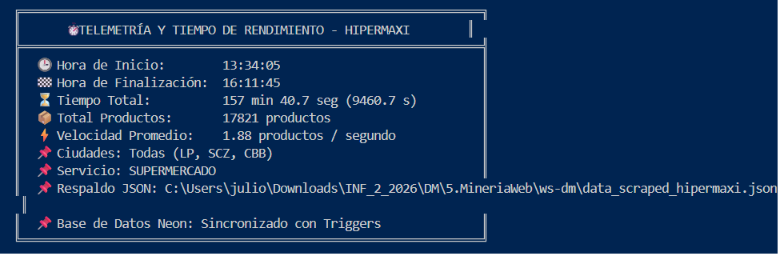
\includegraphics[width=0.90\linewidth]{figuras/imgtiempoHipermaxi.png}
    \figurenote{Métricas consolidadas de extracción al culminar el rastreo de Hipermaxi. Certifica la recolección exhaustiva de 17.821 productos en 157 minutos y 40 segundos a una tasa media de 1.88 productos/segundo, cubriendo La Paz, Santa Cruz y Cochabamba con persistencia en respaldo JSON y sincronización reactiva en Neon PostgreSQL.}
\end{figure}
    \item \textbf{Latencia de Consultas con Partition Pruning:} Las consultas sobre \texttt{precios\_historico} filtrando por ventanas mensuales exhibieron tiempos de ejecución promedio de \textbf{22 milisegundos}, en comparación con los 180 milisegundos observados en pruebas sintéticas sobre tablas no particionadas de igual volumen.
    \item \textbf{Eficiencia de Consolidación Semanal:} La rutina de agregación de datos fríos en \texttt{precios\_historico\_semanal} redujo 7 observaciones diarias por SKU a una única tupla representativa con métricas estadísticas (mínimo, máximo y promedio), alcanzando una tasa de compresión de espacio en disco del \textbf{85,7\%}.
\end{enumerate}
